% !TeX root = ./00.ppgcc-2020.tex

% \chapter{Implementação}\label{cha:implementacao}

% % procedimento experimental previamente definido de ambos, \mfog e da
% % implementação original do algoritmo MINAS, e comparadas.

% % !TeX root = ./00.ppgcc-2020.tex

\subsection{Implementações Preliminares}\label{sec:resultados}

No desenvolvimento parcial desta pesquisa, algumas experimentações e algumas
ferramentas de teste já foram desenvolvidas.
Aspectos desses desenvolvimentos são descritos a seguir.
% obrigado hélio.

\subsubsection{Implementação com \python e \kafka}

A primeira implementação e avaliação do \mfog realizada foi construída sobre a
linguagem \python com o sistema de fila de mensagens \kafka e a respectiva
biblioteca de conexão.
A escolha desse conjunto para a implementação ocorreu \hlhl{devido à ampla}
disponibilidade de bibliotecas de aprendizagem de máquina no ecossistema
\python e, à simplicidade geral da linguagem.
Na implementação desenvolvida, o sistema \kafka recebe mensagens e as armazena
em tópicos distribuídos em partições replicadas em nós de um \cluster,
gerenciados por um nó mestre e suportados pelo serviço de gerenciamento de
configuração distribuída \emph{Apache ZooKeeper}.
A aplicação \emph{Python} consome eventos através da interface \emph{Consumer API},
que expõe a distribuição através da associação de um consumidor às partições
mantidas pelo \kafka.

Para essa implementação, havia a hipótese de que a distribuição de
mensagens gerenciada pelo \kafka
se estenderia a processos consumidores, efetivamente distribuindo o volume de
mensagens entre eles igualmente.
No entanto, a hipótese foi refutada nos experimentos realizados.
Os experimentos em questão foram compostos de 8 processos consumidores, um
processo produtor, uma instância \kafka com 8 partições em seu tópico principal
e uma instância \emph{Apache ZooKeeper} associada à instância \kafka.
% A hipótese era que, como o número de partições igualava o número de consumidores,
% cada consumidor associaria-se a uma partição, distribuindo os dados igualmente
% entre os consumidores para a paralelização a execução.
A hipótese foi refutada quando observou-se que o número de
mensagens consumidas por um dos 8 processos representava a maioria (mais de
80\%) do volume introduzido no sistema, o restante sendo distribuído entre
outros 3 processos e o restante dos processos não recebia nenhuma mensagem.
Portanto, a iniciativa de implementar o algoritmo MINAS em \python com \kafka e
atingir os objetivos de distribuição falhou, o que levou à reconsideração das
plataformas escolhidas.

\subsubsection{Implementação com \flink}

% \nota{citar ferramentas e a escolha só depois do python e kafka}
% \nota{entre flink e spark, outro grupo de pesquisa já está explorando spark}

A segunda alternativa explorada teve por inspiração o trabalho de
\citeonline{Viegas2019} e, como outro grupo de pesquisa já estava explorando
o algoritmo na plataforma \emph{Apache Spark}, a segunda implementação
foi baseada na plataforma \flink.

A plataforma \flink tem modelos de processamento tanto de fluxos como em lotes.
O modelo em lotes é implementado como extensão do modelo de fluxos e, apesar
de não ser foco desse trabalho, mostrou-se útil para a construção do \offline,
já que o conjunto consumido por esse módulo é limitado.

Um desafio encontrado durante o desenvolvimento da implementação do \mfog foi a falta
de bibliotecas na plataforma \flink que disponibilizem versões adaptadas
à plataforma de algoritmos base para o algoritmo MINAS.
Em especial, a ausência dos algoritmos \emph{K-means} e \emph{CluStream}
gerou carga imprevista sobre o processo de desenvolvimento
resultando no atraso do processo de desenvolvimento.

Esta implementação segue a arquitetura descrita na \refsec{descricao} e as
avaliações e resultados esperados descritos neste \refcap{proposta}
referem-se à implementação do \mfog na plataforma \flink.

% % !TeX root = ./00.ppgcc-2020.tex

\section{Implementação com MPI}

The original MINAS algorithm has a companion unpublished implementation (\refminas)
written in Java using MOA library base algorithms such as K-means and CluStream,
but our implementation only used K-means.
Another difference between \refminas and \mfog is the calculus of the cluster radius 
from the distances of elements forming the cluster and the cluster's center.
\refminas uses the maximum distance while \mfog uses the standard deviation
of all distances as described in \cite{Faria2016minas}.

\newcommand{\val}{$\vec{v}\,$\xspace}
The stream formats for input and output are also of note.
As input, the algorithm takes samples (\val), which are a sequence of numbers
with dimension $d$.
In addition to \val, for both training and evaluation, the class
identifier is provided as a single character, along with a unique item identifier
(\emph{uid}), which can otherwise be determined from the sample index in the stream.

As its output, the algorithm returns the original sample \val followed by the
assigned label. Adjustments can easily be made to provide the output results as
a tuple containing \emph{uid} and the assigned label.

% - Reprocessamento dos exemplos utilizados para atualização do modelo:
%   - Muda o comportamento do operador de fluxo de `Map` para `Flatmap`, ou seja,
%     requer outro fluxo de saída para a transmissão de padrões novidade (alarmes);
%   - Para reclassificação a definição de raio é modificada de `r = f * σ` (fator
%     multiplicando desvio padrão) para `r = max(distance)` (distância máxima);
%   - Passível da crítica de *overfitting*. Isto é, este processo pode
%     inflar a métrica de precisão;
%   - **Solução:** *em aberto*;


\begin{algorithm}[htb]
% {\scriptsize
% \begin{multicols}{2}
    % \SetAlgoVlined
    \SetKwProg{Function}{Function}{:}{}
    \SetKwFor{With}{with}{}{}
    \SetKw{continue}{continue}
    % 
    \SetKwData{MEPC}{MEPC}
    \SetKwData{NF}{NF}
    \SetKwData{mpiSize}{mpiSize}
    \SetKwData{mpiRank}{mpiRank}
    \SetKwData{EndOfStream}{EndOfStream}
    % 
    \SetKwInOut{KwParams}{Parameters}
    \KwParams{mpiNodeRank as \mpiRank}
    % 
    \SetKwFunction{Mfog}{Mfog}
    \SetKwFunction{Sampler}{Sampler}
    \SetKwFunction{Classifier}{Classifier}
    \SetKwFunction{Detector}{Detector}
    \SetKwFunction{modelReceiver}{modelReceiver}
    % 
    \SetKwFunction{typeOf}{typeOf}
    % 
    \SetKwFunction{Thread}{Thread}
    \SetKwFunction{Lock}{Lock}
    \SetKwFunction{readLock}{readLock}
    \SetKwFunction{writeLock}{writeLock}
    % 
    \SetKwFunction{receive}{receive}
    \SetKwFunction{send}{send}
    \SetKwFunction{broadcast}{broadcast}
    % 
    \SetKwFunction{nearestCluster}{nearestCluster}
    \SetKwFunction{NoveltyDetection}{NoveltyDetection}
    \SetKwFunction{handleModelSleep}{handleModelSleep}
    \SetKwFunction{removeOldSamples}{removeOldSamples}
    \SetKwFunction{now}{now}
    % 
    \KwIn{ModelSet, Sample Stream}
    % \KwOut{Classified Stream as $out$}
    % 
    \Function{\Mfog{ModelStream, InputStream, OutputStream}}{
        ModelSet = $\emptyset$\;
        ModelSetLock = \textbf{new} \Lock()\;
        \eIf(\emph{root}){\mpiRank == 0}{
            \textbf{new} \Thread(\Detector, [OutputStream, ModelSet, ModelSetLock])\;
            \Sampler(InputStream, ModelSet, ModelSetLock)\;
        }(\emph{leaf}){
            \textbf{new} \Thread(\modelReceiver, [ModelSet, ModelSetLock])\;
            \Classifier(ModelSet, ModelSetLock)\;
        }
    }
\caption{MFOG: main MPI entry-point.}
\label{alg:MFOG}
\end{algorithm}

\begin{algorithm}[htb]
    \SetKwFor{With}{with}{}{}
    \SetKw{continue}{continue}
    % 
    \SetKwData{MEPC}{MEPC}
    \SetKwData{NF}{NF}
    \SetKwData{mpiSize}{mpiSize}
    \SetKwData{mpiRank}{mpiRank}
    \SetKwData{EndOfStream}{EndOfStream}
    % 
    \SetKwProg{Function}{Function}{:}{}
    \Function{\Classifier{ModelSet, ModelSetLock}}{
        \While{ True }{
            sampe = \receive(SampleType, root)\;
            \lIf{sample == \EndOfStream}{\textbf{break}}
            sample.label = unknown\;
            \With{\readLock(ModelSetLock)}{
                (distance, cluster) = \nearestCluster(sample, ModelSet)\;
            }
            \If{distance $<$ cluster.radius}{
                sample.label = cluster.label\;
            }
            \send(root, SampleType, sample)\;
        }
    }
%     \label{alg:MFOG-classifier}
%     \caption{MFOG: Classifier task.}
% \end{algorithm}
% \begin{algorithm}
    % \SetKwProg{algorithm}{algorithm}{:}{}
    \SetKwFor{With}{with}{}{}
    \SetKw{continue}{continue}
    % 
    \SetKwData{MEPC}{MEPC}
    \SetKwData{NF}{NF}
    \SetKwData{mpiSize}{mpiSize}
    \SetKwData{mpiRank}{mpiRank}
    \SetKwData{EndOfStream}{EndOfStream}
    % 
    \SetKwProg{Function}{Function}{:}{}
    \Function{\modelReceiver{ModelSet, ModelSetLock}}{
        \While{ True }{
            cl = \receive(ClusterType, root)\;
            \lIf{cl == \EndOfStream}{\textbf{break}}
            \With{writeLock(ModelSetLock)}{
                ModelSet = ModelSet $\cup$ cl\;
            }
        }
    }
    % \label{alg:MFOG-model}
    % \caption{MFOG: model receiver task.}
\caption{MFOG Leaf Tasks: Model Receiver and Classifier.}
\label{alg:MFOG-leaf}
\end{algorithm}
\begin{algorithm}[htb]
    \SetKwFor{With}{with}{}{}
    \SetKw{continue}{continue}
    % 
    \SetKwData{MEPC}{MEPC}
    \SetKwData{NF}{NF}
    \SetKwData{mpiSize}{mpiSize}
    \SetKwData{mpiRank}{mpiRank}
    \SetKwData{EndOfStream}{EndOfStream}
    \SetKwInOut{KwParams}{Parameters}
    \KwParams{mpiClusterSize as \mpiSize}
    \SetKwProg{Function}{Function}{:}{}
    \Function{\Sampler{InputStream, ModelSet, ModelSetLock}}{
        % ModelSet = read()\;
        % broadcast(ModelSet)\;
        dest = 1\;
        \ForEach{ sample from InputStream }{
            \If{\typeOf(sample) is Cluster}{
                \broadcast(ClusterType, sample, root)\;
                \With{\writeLock(ModelSetLock)}{
                    ModelSet = ModelSet $\cup$ sample\;
                }
                \continue\;
            }
            % sample.label = unknown\;
            \send(dest, SampleType, sample)\;
            dest = dest $+ 1$\;
            \lIf{dest $>$ \mpiSize}{dest = 1}
        }
    }

%     \label{alg:MFOG-sampler}
%     \caption{MFOG: sampler Module.}
% \end{algorithm}
% \begin{algorithm}
    \SetKwProg{algorithm}{algorithm}{:}{}
    \SetKwFor{With}{with}{}{}
    \SetKw{continue}{continue}
    % 
    \SetKwData{cleaningWindow}{cleaningWindow}
    \SetKwFunction{removeOldSamples}{removeOldSamples}
    \SetKwData{noveltyDetectionTrigger}{noveltyDetectionTrigger}
    \SetKwData{MEPC}{MEPC}
    \SetKwData{NF}{NF}
    \SetKwData{mpiSize}{mpiSize}
    \SetKwData{mpiRank}{mpiRank}
    \SetKwData{EndOfStream}{EndOfStream}

    \KwParams{\cleaningWindow, \noveltyDetectionTrigger}

    \SetKwProg{Function}{Function}{:}{}
    \Function{\Detector{OutputStream, ModelSet, ModelSetLock}}{
        lastCleanup $\leftarrow 0$\;
        \While{ True }{
            sampe = \receive(SampleType, any)\;
            \lIf{sample == \EndOfStream}{\textbf{break}}
            % $out \leftarrow$ sample\;
            OutputStream.append(sample)\;
            \If{sample.label == unknown}{
                UnknownSet = UnknownSet $\cup$ sample\;
                \If{$|\;UnknownSet\;| \geq$ \noveltyDetectionTrigger}{
                    novelties = \NoveltyDetection(ModelSet, *UnknownSet)\;
                    \With{\writeLock(ModelSetLock)}{
                        ModelSet = ModelSet $\cup$ novelties\;
                    }
                    \ForEach{ cl in novelties }{
                        \broadcast(ClusterType, cl, root)\;
                    }
                }
                \If{ sampe.uid $ > $ ( lastCleanup $ + $ \cleaningWindow )}{
                    UnknownSet $\leftarrow$ \removeOldSamples(UnknownSet, lastCleanup)\;
                    lastCleanup $ \leftarrow $ sampe.uid\;
                }
            }
        }
    }
    % \label{alg:MFOG-detector}
    % \caption{MFOG: detector task.}
\caption{MFOG Root Tasks: Sampler and Detector.}
\label{alg:MFOG-root}
\end{algorithm}

For evaluation purposes, an \mfog implementation was made using MPI (\emph{Open
MPI 4.0.4}).
The program is organized in a single program multiple data (SPMD)
programming model, so a single version of the \mfog program was initiated on all
nodes, being that one of them would perform the root role, while the others ran
as leaves, the program entry point is illustrated on Algorithm \ref{alg:MFOG}.
On the root process, a sampler thread is responsible for distributing the
sampled flow information (\val) to the classifier nodes, using a round-robin
load balancing scheme.
The other thread on the root process is responsible for receiving the
classification results and for processing the unknown samples in the search for
novelties.
The root process functions are illustrated in Algorithm \ref{alg:MFOG-root}.
Each leaf node runs a model adjustment thread and multiple (up to the number of
cores) classifier threads. The leaf tasks are illustrated in Algorithm
\ref{alg:MFOG-leaf}.
The overall sequence of interactions is shown in Figure \ref{fig:mfog-mpi-life}.

\begin{figure}[htb]
  \centerline{
    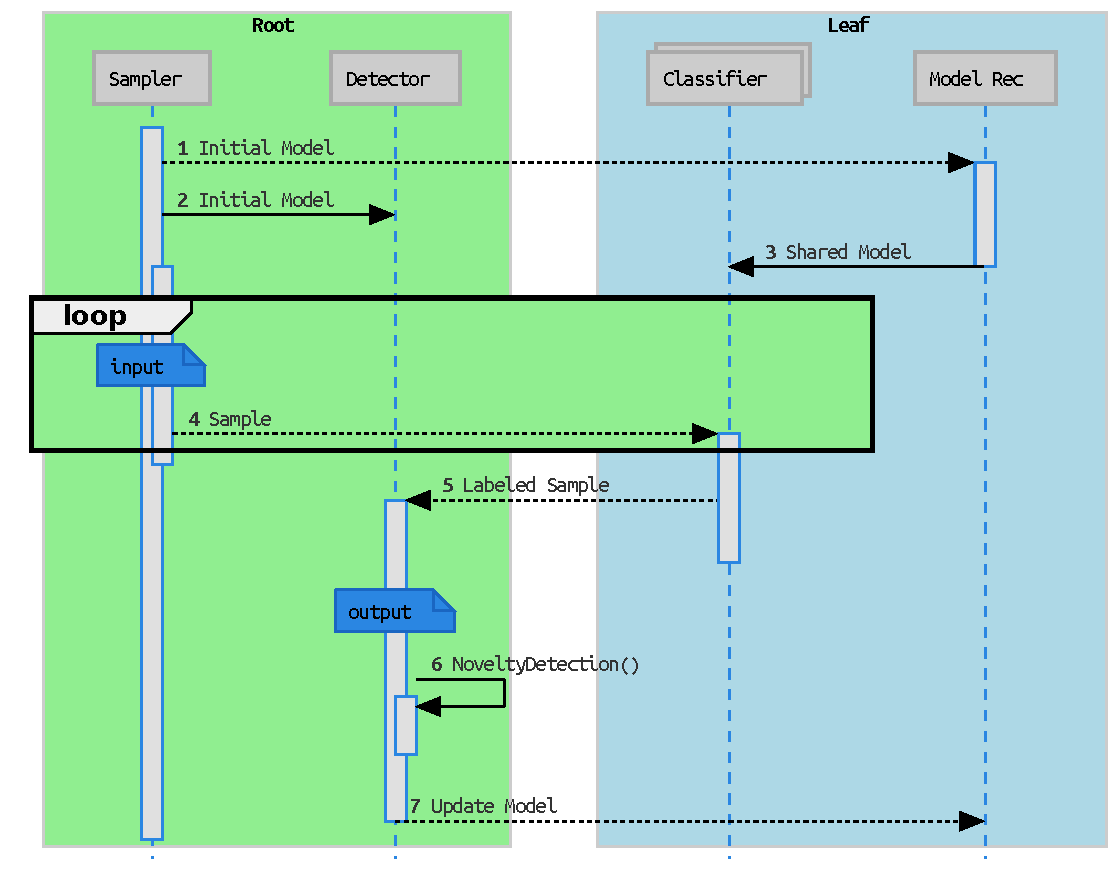
\includegraphics[width=0.75\linewidth,page=1]{figures/lifecycle-uml-svg.pdf}
  }
  \caption{\mfog life line overview.}
  \label{fig:mfog-mpi-life}
\end{figure}


\chapter{Experimentos e Resultados}\label{cha:results}

Este capítulo apresenta o ambiente experimental e os resultados obtidos dos
experimentos, discutindo as métricas de qualidade da classificação e
escalabilidade do \mfog.

% !TeX root = ./00.ppgcc-2020.tex

\section{Ambiente de Teste}\label{sec:ambiente}

Com o objetivo de avaliar esta proposta e averiguar os efeitos da distribuição
da detecção de novidades em um cenário \iot, construiu-se um ambiente
experimental de névoa.

Este ambiente é composto por três computadores de única placa (\emph{Single
Board Computer}) modelo Raspberry Pi 3 model B, equipados com o SoC
(\emph{system-on-chip} - sistema em um chip) de arquitetura ARM \emph{BCM2837} com
$4$ núcleos de processamento à frequência de $1.2\,GHz$, $32\,kB$ e $512\,kB$ de
memória \emph{cache} nível 1 e 2 respectivamente, $1\,GB$ de memória RAM,
armazenamento em cartão SD e conectados por rede cabeada \emph{Ethernet}.
% Switch
% Hélio:
%    Há algo estranho na descrição dos nós; parece que você está misturando nós e cores.
%    Talvez seja mais claro falar do número de nós, ao invés dos cores...
% ficou melhor!

A ideia central é criar um cluster simples simulando \emph{gateway} de uma rede
\iot com recursos limitados.
Este cluster armazenou todo o código-fonte, binários (compilados no mesmo cluster) e
\dataset.
Nesta configuração, o \dataset é armazenado no cartão SD do nó raiz e é lido para
cada execução do experimento.
Todos os experimentos foram executados neste cluster para isolamento de outras
variações imprevistas e para garantir que as comparações seriam justas com
\emph{software} e \emph{hardware} constante.

% The idea was to create a simple cluster simulating an \iot network with
% constrained resources at the edge of the network.
% This cluster stored all source code, binaries (compiled and linked in place) and
% data sets.
% In our setup, the data set is stored in the root's node SD card and is read for
% each experiment.
% All experiments were executed in this cluster for isolation of otherwise
% unforeseen variations and for safe software comparison with constant hardware.
% data sets, being accessed via our laboratory network over Secure Shell (SSH).

O \dataset \emph{Kyoto 2006+}\footnote{Disponível em
\url{http://www.takakura.com/Kyoto\_data/}.}, tráfego das \emph{Honeypots} da
Universidade de Kyoto, é a referência de um cenário real para este trabalho.
% será que é o ``foco''? Talvez é a ``referência de um cenário real''...(?)
Este \dataset contém dados ainda representativos (até 2015) e as característica
desejáveis de um conjunto de dados (realismo, validade, etiquetas previamente
definidas, alta variabilidade, reprodutibilidade e disponibilidade pública) são
atendidas \cite{KyotoDataset,Song2011kyoto}.

O segmento utilizado deste \dataset é o de Dezembro de 2015, contendo $7\:865\:245$ instâncias.
Deste segmento, são mantidas apenas instâncias associadas a tráfego normal ou
a ataques conhecidos, identificados por \nids que tenham mais de $10\,000$ instâncias
para significância, como feito previamente por \citeonline{Cassales2019}.
% , this removes 46,390 instances. TODO: revisar, pois 7M != 700K.
As instâncias mantidas são normalizadas para que o valor de cada característica
original (como endereço IP, duração do fluxo, serviço) seja transposta para o
intervalo Real $[0, 1]$.

O conjunto resultante da operação recém descrita é então dividido em dois
conjuntos, treinamento e teste.
Para avaliar a detecção de ataques, o conjunto treinamento é composto apenas de
tráfego normal, contendo $72\:000$ instâncias.
O conjunto de teste possui $653\:457$ instâncias, sendo elas
$206\:278$ instâncias com classe ``$N$'' (normal) e
$447\:179$ instâncias com classe ``$A$'' (ataque).
%
% Não entendi essa questão de filtrar apenas os ``normal'' class no training set... Hélio
% acho que fez sentido... detectar o que não se aproxima de normal como novidade...

Destaca-se que essa manipulação do \dataset causa \emph{Overfitting} para a classe
normal e \emph{under-fitting} para a classe ataque, pois o sistema primeiro
precisa detectar um padrão novidade para então adicionar ao modelo.
%O foco deste trabalho não é a otimização da detecção de intrusão é contexto de validar metodologia de construcao do \mfog - distribuição e paralelismo em ambiente em \fog.
Como o foco deste trabalho é na arquitetura e metodologia de paralelização e
distribuição em névoa, a otimização do processo de detecção de intrusão não foi
abordada, deixando a questão de escolha do \dataset e do processo de sua manipulação
 em aberto.

Quanto aos parâmetros do algoritmo \minas, ilustrados na Figura
\ref{fig:params}, os valores foram escolhidos por \hlke{serem valores comuns para o
algoritmo presentes na literatura} \cite{Faria2013Minas,Faria2016minas} e na
implementação de referência \refminas \cite{Faria2013source}.
Os parâmetros que não tem valores comuns na literatura foram escolhidos e ajustados até os
os resultados obtidos se aproximarem aos resultados da implementação de referência \refminas.

\begin{figure}[htb]
  \centering
  \begin{lstlisting}
    MinasParams minasParams = {
      .k=100, .dim=22, .precision=1.0e-08,
      .radiusF=0.25, .minExamplesPerCluster=20, .noveltyF=1.4,
      .thresholdForgettingPast = 10000,
    };
  \end{lstlisting}
  \caption{Parâmetros do algoritmo \minas.}
  \label{fig:params}
\end{figure}

Os parâmetros utilizados da literatura são
\texttt{k}, que é o número de \mclusters gerados pelo algoritmo de agrupamento,
\texttt{minExamplesPerCluster}, que indica o número mínimo de exemplos para um
\mcluster válido (representatividade) e,
\texttt{thresholdForgettingPast}, que estabelece o limite para remoção de exemplos do conjunto de
desconhecidos.

Os parâmetros escolhidos por aproximação de resultados são:
\texttt{precision}, que é o valor limite para melhora na distância global reduzindo as 
iterações no algoritmo de agrupamento (otimização),
\texttt{radiusF}, que corresponde ao fator que multiplica o desvio padrão das distâncias entre o
centro e cada exemplo formador do novo \mcluster definindo o raio do \mcluster
e,
\texttt{noveltyF}, que é o fator que multiplica o desvio padrão das distâncias do
\mcluster mais próximo distinguindo um novo padrão entre extensão e novidade.

% (k, minExamplesPerCluster, noveltyF, thresholdForgettingPast)
% (precision, radiusF)

% Para realização dos experimentos, diversas configurações de ambientes são
% propostas.
% Os ambientes selecionados são: local, 
% \notahl{o que muda na paralelização e na \textbf{distribuição} de instâncias
% do módulo \textbf{classificador}?}
% \hlhl{nuvem e névoa}.
% As configurações consistem na distribuição de módulos da implementação \mfog
% sendo executadas em combinações de ambientes nuvem e névoa com variada
% quantidade de nós.
  % dá-lhe Yoda! Hélio

% O ambiente local é composto por um único nó computacional, consistindo de um
% computador pessoal equipado com um processador de 8 núcleos, $16GB$ de memória e
% armazenamento em estado sólido (SSD) usado para o desenvolvimento e referência
% em comparações.
% O ambiente nuvem é provido pela utilização da infraestrutura de nuvem da
% Universidade Federal de São Carlos (Cloud{@}UFSCar\footnote{Disponível em
% \url{http://portalcloud.ufscar.br/servicos}}).
% O ambiente de névoa (\fog) é composto por computadores de única placa
% (\emph{Single Board Computer}) equipados com processador de arquitetura ARM de 4
% núcleos, $1GB$ de memória, armazenamento em cartão SD (\emph{SD-card}) e
% conectados por rede sem fio.

% A combinação de diferentes formas de distribuição dos nós tem por objetivo \hlhl{demonstrar padrões de
% latência} e qualidade que podem afetar implantações em ambientes reais que não
% são geralmente destacados quando os experimentos são realizados em um único
% nó ou ambiente.

% Faz parte também do ambiente de teste os conjuntos de dados (\datasets)
% \emph{KDD99}
% % \hlfa{e \emph{Kyoto 2006+}}
% e \emph{Kyoto 2006+}
% que foram selecionados por motivos distintos.

% O \dataset \emph{Kyoto 2006+} é o foco deste trabalho, pois contém dados ainda
% representativos (até 2015) e as característica desejáveis de um conjunto de
% dados (realismo, validade, etiquetas previamente definidas, alta variabilidade,
% reprodutibilidade e disponibilidade pública) são atendidas
% \cite{KyotoDataset,Song2011kyoto}.

% O \dataset \emph{KDD99} é amplamente utilizado em trabalhos de detecção de
% anomalia.
% Porém, como não possui mais a característica de realismo, uma vez que foi
% construído em 1998, neste trabalho o \dataset \emph{KDD99} é utilizado somente
% para que o leitor possa comparar com outros trabalhos
% \cite{Tavallaee2009,Protic2018KddKyoto}.

% Os dois \datasets mencionados e outros abordados em discussão e avaliados como
% relevantes são

% Por exemplo, o KDD original tem 41 atributos. A base é rotulada para 24
% tipos de ataques divididos em 4 grupos: DOS ...
% 
% O paper que analisou a fundo o KDD99 foi este: 
% 
% M. Tavallaee, E. Bagheri, W. Lu, and A. Ghorbani, “A detailed analysis
% of the KDD Cup 1999 data set,” in Proc. 2nd IEEE Symp. Comput. Intell.
% Secur. Defense Appl., 2009, pp. 1–6.
% 
% Qual é o defeito dele? tem muitos dados replicdos tanto na base de
% treinamento quento na de teste, o que gera viés nos resultados. Para
% resolver isso propuseram o NSL-KDD que é um subconjunto do KDD que evita
% esse problema

% \notake{
%   CICIDS2017 {https://www.unb.ca/cic/datasets/ids-2017.html} e
%   ISCXTor2016 {https://github.com/ahlashkari/CICFlowMeter}
% }
% \notafa{Uma sugestão seria usar datasets artificiais também a fim de avaliar
% outras caracteristicas tais como: nro de atributos, frequencia do surgimento de
% novidades, mudanças abruptas, graduais, etc. }
% \begin{table}[ht]
%   \caption{Sumário dos conjuntos de dados}
%   \centering
%   \begin{scriptsize}
%   \begin{tabularx}{\linewidth}{X|X|X|X}
%     Nome &
%       Origem &
%       Descrição &
%       Acesso Público \\
%     \hline
%     \hline
%     \emph{KDD99} \cite{Tavallaee2009,Protic2018KddKyoto} &
%       Captura de Fluxos de rede com ataques simulados &
%       41 atributos (sumário de fluxo), 23 classes, $4\;898\;431$ instâncias, $709$ MB &
%       \url{https://kdd.ics.uci.edu/databases/kddcup99/kddcup99.html} \\
%     \hline
%     \emph{Kyoto 2006+} \cite{Song2011kyoto,Protic2018KddKyoto}&
%       Captura de Fluxos de rede com HoneyPot &
%       23 atributos (sumário de fluxo), 3 classes, $7\;865\;245$ instâncias e $1.3$ GB (dez-2015) &
%       \url{https://www.takakura.com/Kyoto_data/new_data201704/} \\

%       %  0.000000 other 0 0 0 0.00 0.00 0.00 0 0 0.00 0.00 0.00 S0 00 0 -1
%       %  fdbd:f115:35b2:0424:40aa:098c:03e5:149b 3712
%       %  fdbd:f115:35b2:c891:7db9:2762:6182:03eb 445 00:00:00 tcp
    
%        \hline
%     % ISCXTor2016 \cite{Draper-Gil2016} &
%     %   Origem &
%     %   28 atributos,  &
%     %   \url{https://www.unb.ca/cic/datasets/tor.html} \\
%     % \hline
%     % ISCXVPN2016 \cite{Lashkari2017} &
%     %   Origem &
%     %   28 atributos,  &
%     %   \url{https://www.unb.ca/cic/datasets/tor.html} \\
%     % \hline
%     CICIDS2017 \cite{Sharafaldin2018cicids2017} &
%       Captura de Fluxos de rede com ataques simulados com perfil de trafego de 25
%       usuários normais e de 6 perfis de ataques durante 5 dias (1º dia sem ataque) &
%       80 atributos (sumário de fluxo extraído de CICFlowMeter), 15 classes,
%       $2\;830\;751$ instâncias e 1.2GB em arquivos \emph{pcap} e \emph{csv} &
%       \url{https://www.unb.ca/cic/datasets/ids-2017.html} \\
%     \hline
%     \emph{Radial Basis Function} (RBF) da biblioteca \emph{Massive Online Analysis} (MOA)
%     \emph{4CRE-V2} &
%       Sintético gerado por função RBF da biblioteca MOA com características de
%       mudança e evolução de conceito &
%       Atributos ($\mathbb{R}$), exemplos, classes, evoluções e mudanças configuráveis &
%       \url{https://sites.google.com/site/nonstationaryarchive/home} \\
%     \hline
%   \end{tabularx}
%   \label{tab:summary-dataset}
%   \end{scriptsize}
% \end{table}


% \input{54.experimentos.tex}

% \FloatBarrier
\section{Experimentos, Métricas e Visualizações}
\label{sec:experiments}
% acho que convém explicar as demais tabelas de resultados...

\newcommand{\expA}{\textit{a-Referência}\xspace}
\newcommand{\expB}{\textit{b-Sequencial}\xspace}
\newcommand{\expC}{\textit{c-Paralelo}\xspace}
\newcommand{\expD}{\textit{d-Distribuído}\xspace}

Seguindo as especificações de ambiente da Seção \ref{sec:ambiente}, cada
experimento consiste na execução de um dos programas ((a)\minas referência 2013
\cite{Faria2013source}, (b) implementação sequencial do \minas com a nova
biblioteca, (c) \mfog em um ou (d) três nós) com variação do parâmetro de paralelismo,
fornecendo um modelo inicial e \dataset de teste como fluxo de entrada e
capturando o fluxo de saída para e extração das métricas estabelecidas na Seção
\ref{sec:avaliacao}.
Destes experimentos, listados na Tabela \ref{tab:exp-list}, os seguintes
resultados são apresentados.

\begin{table}[htb]
  \centering
  % \setlength\tabcolsep{0.5em}
  \caption{Listagem dos principais experimentos.}
  \label{tab:exp-list}
  \begin{tabular}{p{0.17\textwidth}|p{0.27\textwidth}|p{0.47\textwidth}}
  \textbf{Experimento} & \textbf{Programa}                 & \textbf{Características} \\\hline
  \expA                & \minas referência 2013            & Raio é a distância máxima. \\\hline
  \expB                & \minas sequencial para validação  & 
    Raio é o desvio padrão das distâncias;
    Modelo único;
    Remoção de desconhecidos mais agressivo. \\\hline
  \expC                & \mfog 1 nó, 4 processadores       & 
    Classificadores paralelos;
    Detecção de novidade assíncrona. \\\hline
  \expD                & \mfog 3 nós, 12 processadores     &
    Mais processadores;
    Comunicação em rede.
  \end{tabular}
  \end{table}

\subsection{Validação do algoritmo}

Para validar a biblioteca de funções do \mfog que implementa o algoritmo \minas,
uma versão do Algoritmo \ref{alg:minas-main} foi construída, sem classificadores
paralelos ou detecção de novidade assíncrona, aspectos que caracterizam o \mfog.
Esta implementação utiliza a definição de raio da Equação \ref{eq:raio_paper}
(desvio padrão das distâncias).
Feita esta implementação foram realizados os experimentos \expB com esta
implementação e \expA com a implementação \minas referência.
Estes dois experimentos utilizam apenas um nó e um processador do ambiente
experimental, sendo que as métricas são extraídas conforme a \refsec{avaliacao}
e são comparadas nesta Subseção, mostrando a equivalência entre as implementações.

A Tabela \ref{tab:java-matrix} mostra a matriz de confusão no instante final do
fluxo de saída do experimento \expA.
Nesta matriz, o rótulo ``desconhecido'' é o caractere ``$-$'' e os valores de
associação e verdadeiro-positivo estão atrelados à coluna de cada rótulo; no
demais a matriz segue os atributos definidos na Seção \ref{sec:avaliacao}.
Esta matriz é comparada com a matriz de confusão do mesmo instante do fluxo de
saída do experimento \expB, e os resultados são apresentados na Tabela \ref{tab:libc-matrix}.

\begin{table}[hbt]%{\linewidth}
  {\footnotesize
  % \setlength\tabcolsep{0.5em}
  \begin{center}
  \caption{Experimento \expA, Matriz de confusão do \dataset \emph{Kyoto} Dez. 2015.}
  \label{tab:java-matrix}
  \begin{tabular}{l *{14}{|r} }
    Rótulos   &     - &       N &    1 &    2 &    3 &  4 &   5 &    6 &    7 &     8 &    9 &    10 &   11 &  12 \\\hline
    Classes  &       &         &      &      &      &    &     &      &      &       &      &       &      &     \\\hline
    \hline
    A        &  3\;774 &  438\;750 &  123 &  145 &  368 &  8 &  52 &  165 &    1 &  1\;046 &  161 &  2\;489 &   71 &  26 \\\hline
    N        &  8\;206 &  193\;030 &    0 &   79 &   44 &  0 &   0 &    0 &  229 &   181 &  154 &  4\;066 &  289 &   0 \\\hline
    \hline
    Associação &     - &       N &    A &    A &    A &  A &   A &    A &    N &     A &    A &     N &    N &   A \\\hline
    Hits ($tp$)     &     0 &  193\;030 &  123 &  145 &  368 &  8 &  52 &  165 &  229 &  1\;046 &  161 &  4\;066 &  289 &  26 
  \end{tabular}
\end{center}
}
\end{table}

Comparando as duas matrizes, a primeira diferença aparente é o índice do
primeiro rótulo novidade ($0$ ao invés de $1$), mas isso se deve apenas à decisão
arbitrária.
% A sentença a seguir está bem longa, difícil de acompanhar. Fragmentar?
A primeira diferença notável que influi nas métricas de qualidade é a falta de 3
rótulos novidade, $12$ rótulos no experimento \expA e $9$ no experimento \expB,
seguido do número de exemplos desconhecidos, $28\,567$ no experimento \expB e
$11\,980$ no experimento \expA e, o montante de exemplos incluídos nos rótulos
novidade, muito menor no experimento \expB.

\begin{table}[hbt]%{\linewidth}
  % {\small
  % \setlength\tabcolsep{0.5em}
  \begin{center}
  \caption{Experimento \expB, Matriz de confusão do \dataset \emph{Kyoto} Dez. 2015.}
  \label{tab:libc-matrix}
  \begin{tabular}{l|r|r|r|r|r|r|r|r|r|r|r}
    Rótulos &      - &       N &   0 &    1 &    2 &   4 &   5 &  6 &   7 &   8 &  10 \\\hline
    Classes  &        &         &     &      &      &     &     &    &     &     &     \\\hline
    \hline
    A        &  16\;086 &  429\;765 &  94 &  995 &  104 &   0 &  23 &  3 &  29 &  46 &  34 \\\hline
    N        &  12\;481 &  193\;642 &   3 &   94 &    0 &  47 &   0 &  0 &   0 &  11 &   0 \\\hline
    \hline
    Associação &      - &       N &   A &    A &    A &   N &   A &  A &   A &   A &   A \\\hline
    Hits ($tp$)     &      0 &  193\;642 &  94 &  995 &  104 &  47 &  23 &  3 &  29 &  46 &  34 
  \end{tabular}
  \end{center}
  % }
\end{table}

Estas três diferenças são atribuídas à divergência entre as definições de raio
discutidas na Seção \ref{sec:minas-og}, Equações \ref{eq:raio_max} e
\ref{eq:raio_paper}.
Esta divergência, apesar de inicialmente pequena, muda muito o comportamento do
passo de classificação, resultando em um conjunto diferente de desconhecidos e, 
por fim, mudando muito o resultado da detecção de novidades.
Adicionalmente, como o parâmetro $f_{raio}$ (\texttt{radiusF}) não existe na
versão com raio definido como distância máxima (Eq. \ref{eq:raio_max}), este
parâmetro foi escolhido experimentalmente observando os resultados durante a
implementação.

Além das matrizes de confusão que dão uma visão detalhada, porém somente sobre o
último instante do fluxo, pode-se comparar as visualizações de fluxo onde as
métricas de qualidade são apresentadas para todo o fluxo.
As Figuras \ref{fig:validation-java} e \ref{fig:validation-serial} ilustram os
fluxos de saída dos experimentos \expA e \expB respectivamente.

\begin{figure}[htb]
  \centering
  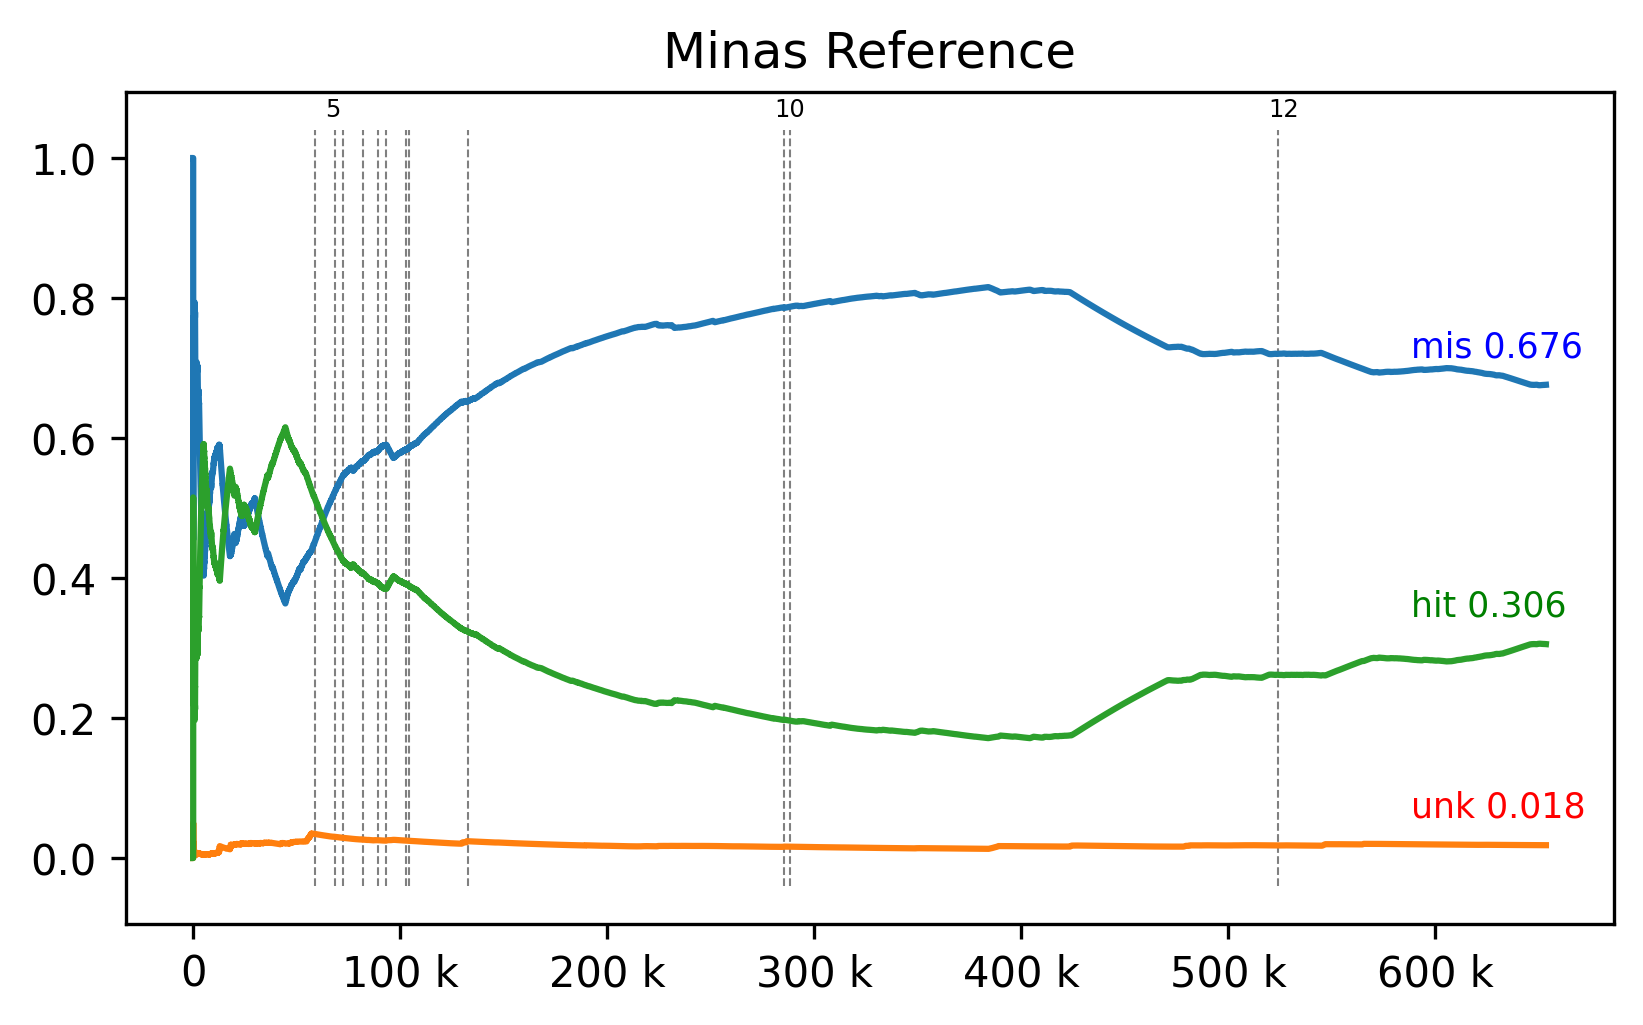
\includegraphics[width=0.75\linewidth]{experiments/revised-java-log.png}
  \caption{Experimento \expA, visualização de fluxo do \dataset \emph{Kyoto} Dez. 2015.}
  \label{fig:validation-java}
\end{figure}

As Figuras \ref{fig:validation-java} e \ref{fig:validation-serial} reforçam a
observação anterior de que mais rótulos novidade (linhas tracejadas verticais
com rótulo no topo) foram encontrados no experimento \expA do que as encontradas 
no experimento \expB.
Outro aspecto com relação a rótulos novidade, no experimento \expA eles surgem
mais ``cedo'' no fluxo, sendo a primeira marcação em $x=58\,967$ contra $x=94\,155$ no
experimento \expB.

\begin{figure}[htb]
  \centering
  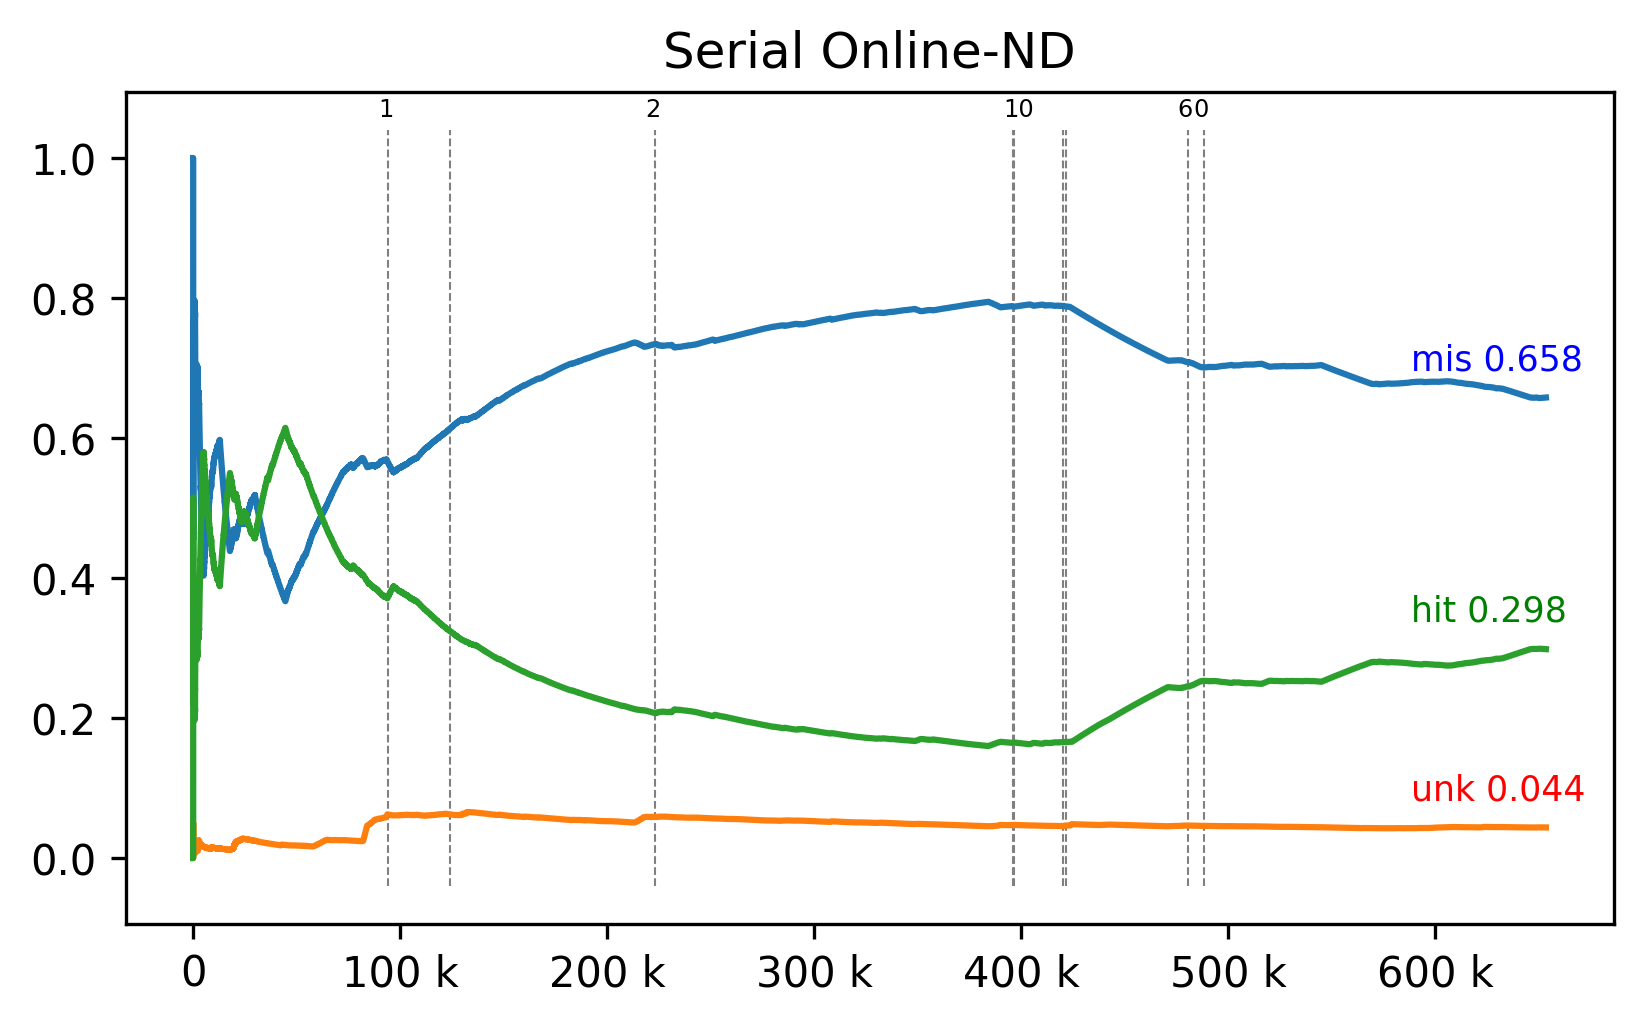
\includegraphics[width=0.75\linewidth]{experiments/online-nd-log.png}
  \caption{Experimento \expB, visualização de fluxo do \dataset \emph{Kyoto} Dez. 2015.}
  \label{fig:validation-serial}
\end{figure}

O gráfico de visualização do fluxo tem no eixo horizontal (x, domínio) o índice
do exemplo $x$ e o eixo vertical (y, imagem) mostra o valor das métricas de qualidade
calculadas até aquele índice de exemplo $x$ no fluxo de saída capturado.
As linhas horizontais na visualização de fluxo mostram o progresso das métricas
de qualidade de classificação durante o fluxo e, ao final na esquerda, o valor
impresso junto e de mesma cor da linha é o valor final de cada métrica.
As métricas são: 
em laranja a taxa de desconhecidos (\texttt{unk}),
em verde a acurácia (\texttt{hit}) e
em azul o erro (\texttt{err}).
Estas métricas podem ser arranjadas em uma tripla-sumário
(\texttt{unk}, \texttt{hit}, \texttt{err})
com os valores em pontos percentuais para fácil comparação.

% Por último, o gráfico de visualização do fluxo mostra as métricas de qualidade
% resumida (\ emph {Acessos}, \ emph {Desconhecidos}, \ emph {Erros}) computada
% para cada exemplo no fluxo de saída capturado. Este resumo é calculado para cada
% exemplo, mas usa a linha \ emph {Atribuída} calculada anteriormente para avaliar
% \ emph {Acertos}; as outras medidas são derivadas conforme descrito antes. 

% Lastly, the stream visualization chart shows the summary quality measurement
% (\emph{Hits}, \emph{Unknowns}, \emph{Misses})
% computed for each example in the captured output stream.
% This summary is computed for each example, but it uses the \emph{Assigned} row
% computed previously to evaluate \emph{Hits}; the other measurements are derived as
% described before.
% The Horizontal axis (x, domain) plots the index of the example and the
% vertical axis (y, image) shows the measurement computed until that example index on the captured
% output stream.

Em conclusão das métricas de qualidade de classificação, os experimentos \expA e
\expB não são idênticos, pois não implementam a mesma definição para o raio,
porém são equivalentes em seus resultados.
Enquanto o experimento \expA tem tripla-sumário
($1.8\%,\: 30.6\%,\: 67.6\%$),
o experimento \expB piora marginalmente nas métricas com
($4.4\%,\: 29.8\%,\: 65.8\%$),
tendo mais desconhecidos, menor acurácia e menor erro.

Para as métricas de escalabilidade, os experimentos \expA e
\expB servem somente como base
para os próximos experimentos onde o paralelismo passa a ser utilizado.
Uma última nota quanto ao tempo de execução, mesmo não sendo paralelo, as
otimizações de memória, redução do uso de \emph{strings} e condição de parada do
algoritmo \emph{K-Means}, reduziram o tempo utilizado pela implementação de
referência de $2\;772s$ ($917s$ \emph{offline} e $1\;845s$ \emph{online}) para
$287s$ ($194s$ \emph{offline} e $93s$ \emph{online} no experimento \expB) na
nova implementação.

\subsection{Paralelismo e Distribuição}
\label{subsec:parallel-dist}

% For the measurements summary table, six measurements from two sources are displayed. Three
  % measures \emph{Hits}, \emph{Unknowns} and \emph{Misses} represented as ratio of
  % the captured output stream, extracted from the evaluation python program,
  % computed as follows:
  % \emph{Hits} (true positive rate) is the sum of the \emph{Hits} row in the
  % extended confusion matrix;
  % \emph{Unknowns} is the count of examples in the captured output stream marked
  % with the \emph{unknown} label (\emph{``-''});
  % \emph{Misses} is the count of all examples in the captured output stream marked
  % with a label distinct from the \emph{Assigned} original class and are not marked
  % as unknown.

  % Furthermore in the measurement summary table, \emph{Time}, \emph{System} and \emph{Elapsed}
  % represented in seconds, are extracted from \emph{GNU Time 1.9}.
  % \emph{Time} is the amount of CPU seconds expended in user-mode
  % (indicates time used doing CPU intensive computing, e.g., math);
  % \emph{System} is the amount of CPU seconds expended in kernel-mode
  % (for our case, it indicates time doing input or output);
  % \emph{Elapsed} is the real-world (wall clock) elapsed time and
  % indicates how long the program took to complete.
  % The lower the times, the better.
  % Our four main experiments are shown in Tab. \ref{tab:exper-summary}.

  % Lastly, the stream visualization chart shows the summary quality measurement
  % (\emph{Hits}, \emph{Unknowns}, \emph{Misses})
  % computed for each example in the captured output stream.
  % This summary is computed for each example, but it uses the \emph{Assigned} row
  % computed previously to evaluate \emph{Hits}; the other measurements are derived as
  % described before.
  % The Horizontal axis (x, domain) plots the index of the example and the
  % vertical axis (y, image) shows the measurement computed until that example index on the captured
  % output stream.

  % Adding to the stream visualization chart, novelty label markers are represented
  % as vertical lines indicating \emph{when} in the captured output stream a new
  % label first appeared.
  % Some of the novelty label markers include the label itself ($l \in \mathbb{N}$)
  % for reference (showing every label would turn this feature unreadable due
  % to overlapping).
  % Figure \ref{fig:visualization} shows complete stream visualization charts.

  % \begin{table*}[htb]
  % \caption{Confusion Matrixes and Qualitative measurements}
  % \label{tab:confusion-matrixes-ref-serial}

% \vspace{3ex}

Seguindo as comparações, para avaliar a escalabilidade dos sistemas, foram
realizados dois experimentos que seguem o mesmo roteiro, o experimento \expC (1 nó e
4 núcleos) e o experimento \expD (3 nós e 12 núcleos).
As Tabelas \ref{tab:single-matrix} e \ref{tab:multi-matrix} mostram as matrizes
de confusão dos experimentos \expC e \expD respectivamente.

\begin{table}[hbt]
  \centering
  % \setlength\tabcolsep{0.5em}
  \caption{Experimento \expC, \mfog com 1 nó e 4 núcleos, Matriz de confusão do \dataset \emph{Kyoto} Dez. 2015.}
  \label{tab:single-matrix}
  \begin{tabular}{l|r|r|r|r|r|r|r}
    Rótulos &      - &       N &    0 &    1 &   2 &  3 &  4 \\\hline
    Classes  &        &         &      &      &     &    &    \\\hline
    \hline
    A        &  12\;282 &  433\;797 &  147 &  952 &   0 &  0 &  1 \\\hline
    N        &   3\;088 &  203\;019 &   40 &   99 &  27 &  5 &  0 \\\hline
    \hline
    Associação &      - &       N &    A &    A &   N &  N &  A \\\hline
    Hits ($tp$)     &      0 &  203\;019 &  147 &  952 &  27 &  5 &  1 
  \end{tabular}
\end{table}

A tripla-sumário do experimento \expC é ($2.4\%,\: 31.2\%,\: 66.4\%$), com menos
desconhecidos em relação ao experimento \expB ($4.4\%,\: 29.8\%,\: 65.8\%$),
sendo esta redução de $2\%$ distribuída $1.4\%$ em acurácia e $0.6\%$ em erro,
representando melhora marginal em todas as métricas.
% há algo estranho nesta frase, parece que falta uma vírgula ou conjunção...

Comparando as matrizes dos experimentos \expB e \expC, observa-se os
efeitos do paralelismo de classificadores e, mais importante, a execução
assíncrona da tarefa de detecção de novidade.
O impacto principal é a redução no número de rótulos novidade, de $9$ para $5$.
Comparando a visualização de fluxo, Figuras \ref{fig:validation-serial} e
\ref{fig:single-flow}, observa-se também que a aparição do primeiro padrão
novidade acontece mais ``tarde''; enquanto em \expB o rótulo novidade ``1'' é
observado em $x = 94\:155$, em \expC o mesmo rótulo é observado em $x =
172\:917$.

Esse comportamento é devido à detecção de novidade assíncrona, pois enquanto
essa tarefa é executada os classificadores continuam utilizando o modelo antigo.
Além disso, como já foi elencado na Seção \ref{sec:polices} item
\ref{reclassification}, os exemplos utilizados para formar o novo \mcluster
com rótulo novidade não são recolocados no fluxo de saída para nova análise.
Estas duas características do \mfog acarretam em um atraso significativo entre a
aparição de um padrão no fluxo de entrada e a aparição do rótulo correspondente
no fluxo de saída.
Em outras palavras, o fluxo avança com o modelo antigo e, mesmo após atualizado,
só gera uma saída com o rótulo novo quando (e se) o padrão aparece novamente.
Este é um resultado muito importante para compreender os problemas relacionados
à distribuição de um algoritmo deste gênero.

\begin{table}[hbt]
  \centering
  % \setlength\tabcolsep{0.5em}
  \caption{Experimento \expD, \mfog com 3 nós de 4 núcleos cada, Matriz de confusão do \dataset \emph{Kyoto} Dez. 2015.}
  \label{tab:multi-matrix}
  \begin{tabular}{l|r|r|r|r|r|r|r}
    Rótulos   &      - &       N &    0 &    1 &    2 &    3 &  4 \\\hline
    Classes   &        &         &      &      &      &      &    \\\hline
    \hline
    A      &  12\;378 &  433\;631 &  117 &  886 &    0 &  162 &  5 \\\hline
    N      &   3\;121 &  202\;916 &   40 &   96 &  105 &    0 &  0 \\\hline
    \hline
    Associação   &      - &       N &    A &    A &    N &    A &  A \\\hline
    Hits ($tp$)   &      0 &  202\;916 &  117 &  886 &  105 &  162 &  5 
  \end{tabular}
\end{table}

Avançando para o experimento \expD, a matriz de confusão na Tabela
\ref{tab:multi-matrix}, mostra pouca diferença quando comparado ao experimento
\expC, com o número de desconhecidos sofrendo a maior variação.

O mesmo é observado quando compara-se a visualização de fluxo, Figuras
\ref{fig:single-flow} e \ref{fig:multi-flow}, há pouca diferença e a tripla-sumário
($2.4\%,\: 31.2\%,\: 66.4\%$) é idêntica.

\begin{figure}[htb]
  \centering
  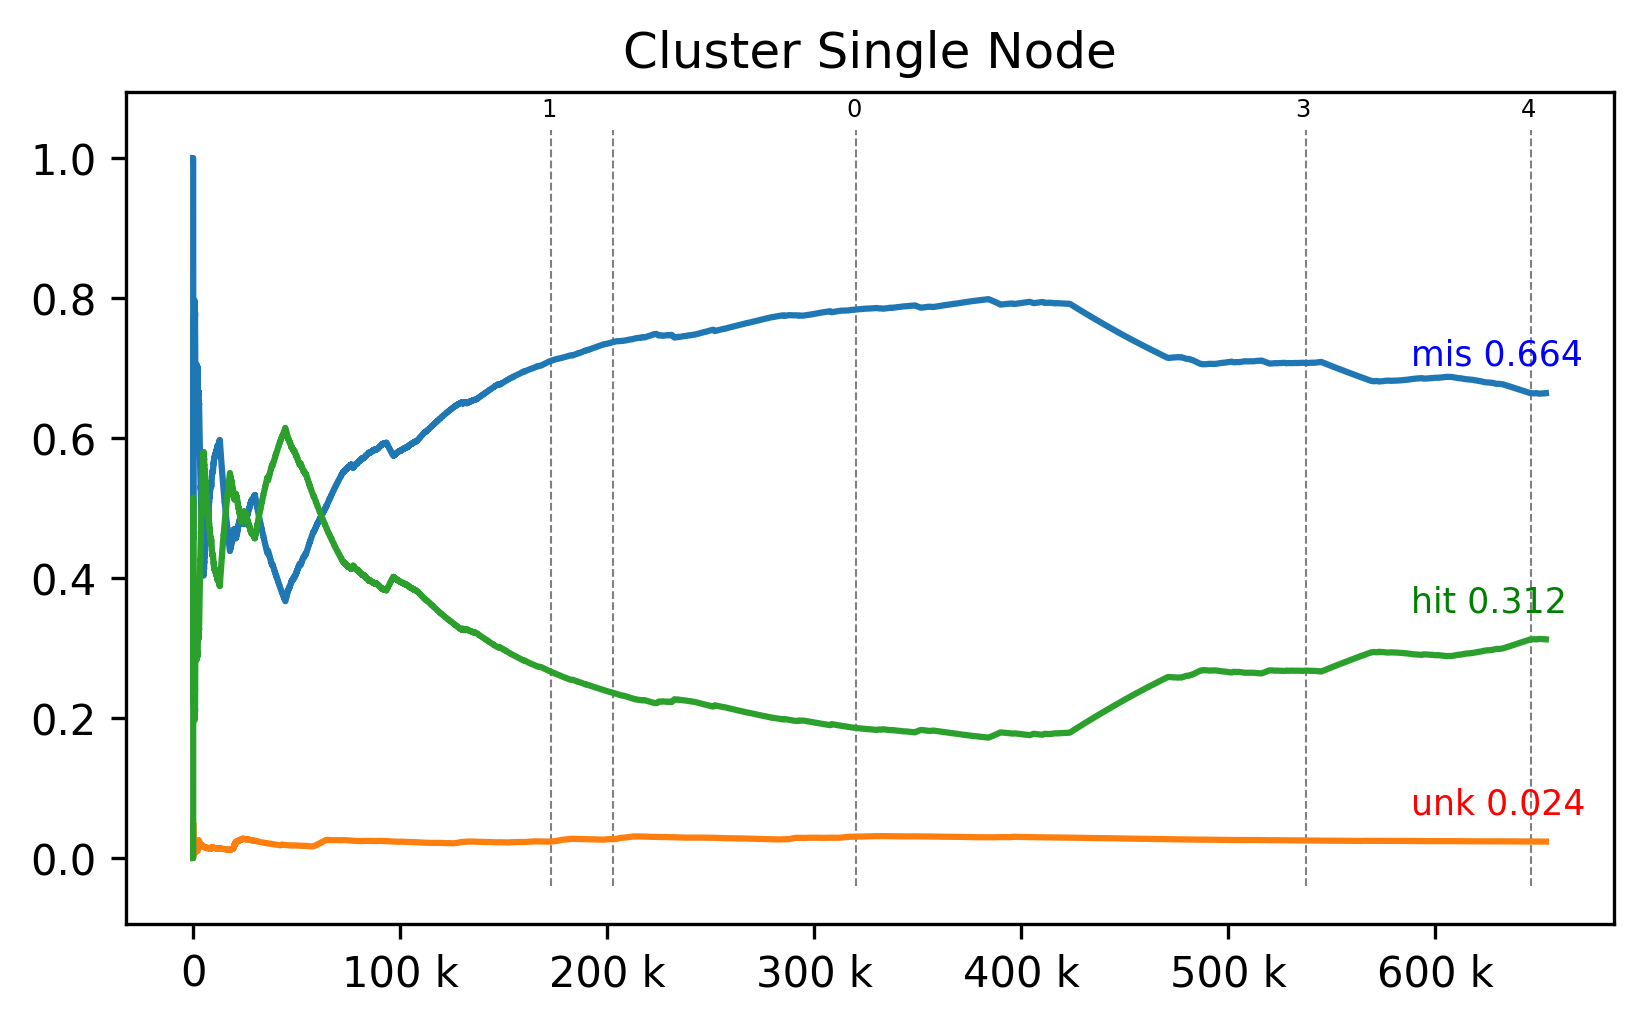
\includegraphics[width=0.75\linewidth]{experiments/tmi-base-log.png}
  \caption{Experimento \expC, \mfog com 1 nó e 4 núcleos, visualização de fluxo do \dataset \emph{Kyoto} Dez. 2015.}
  \label{fig:single-flow}
\end{figure}

\begin{figure}[htb]
  \centering
  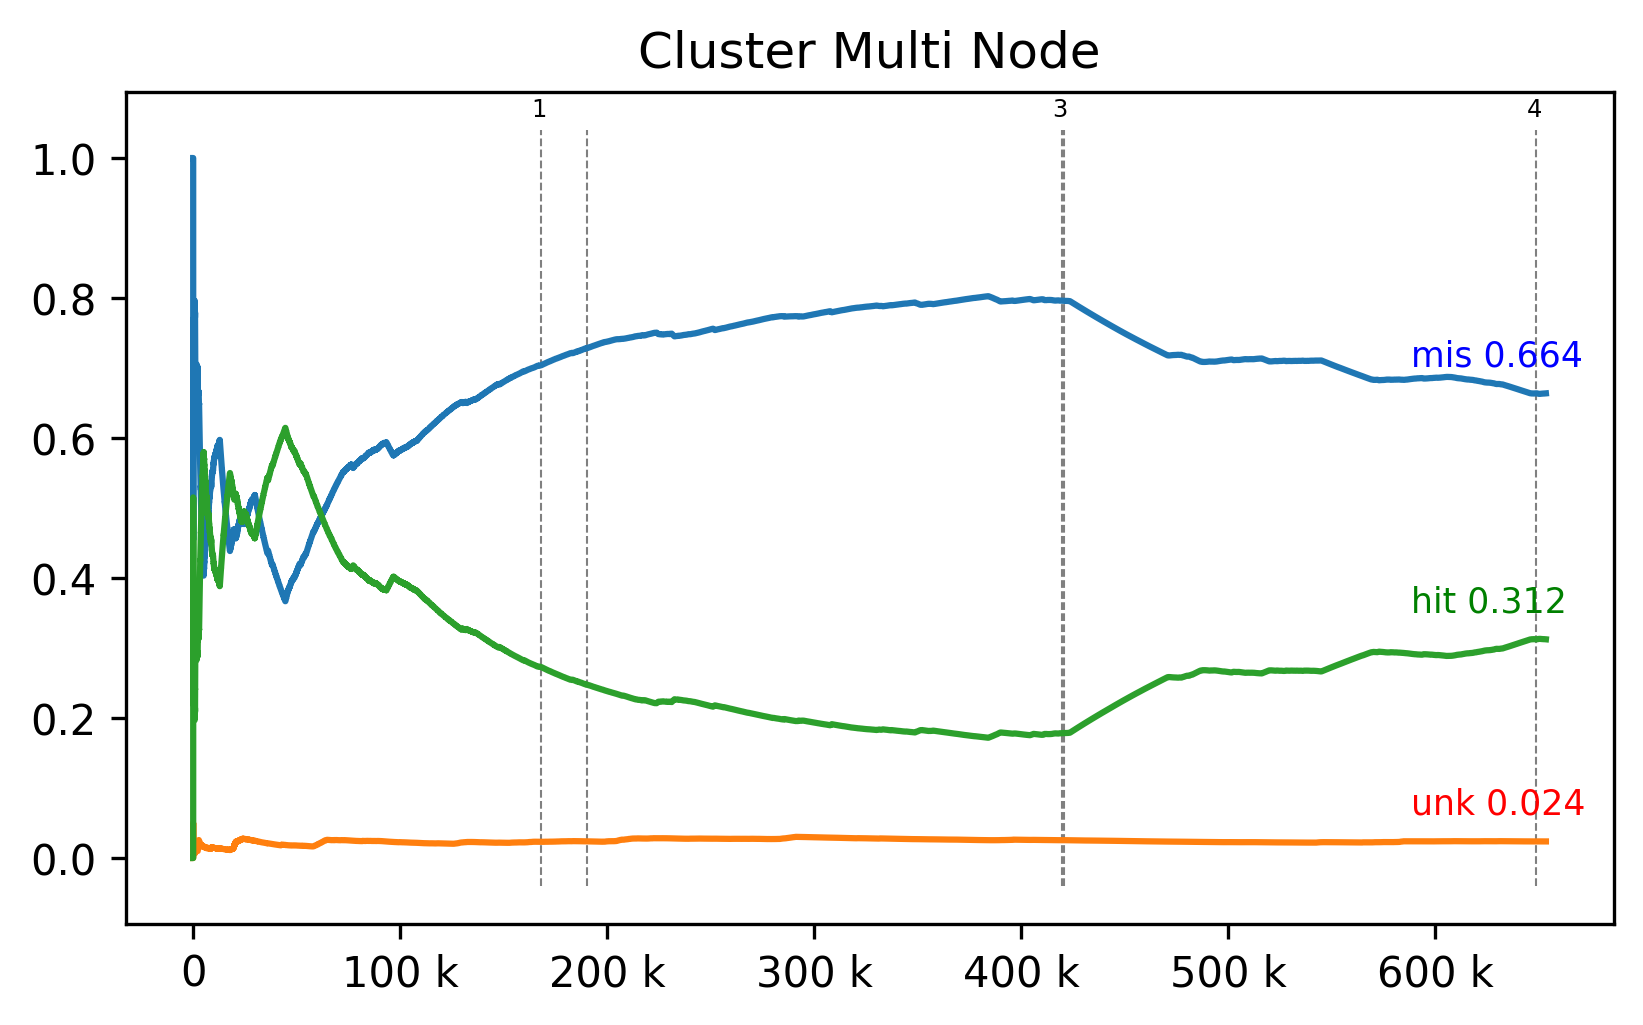
\includegraphics[width=0.75\linewidth]{experiments/tmi-n12-log.png}
  \caption{Experimento \expD, \mfog com 3 nós de 4 núcleos cada, visualização de fluxo do \dataset \emph{Kyoto} Dez. 2015.}
  \label{fig:multi-flow}
\end{figure}

Isto reforça a ideia de que o maior impacto nas métricas de qualidade de
classificação é a mudança de detecção de novidade assíncrona, pois mesmo com o
triplo de instâncias classificadoras, as métricas continuam idênticas.

Com a discussão das métricas de qualidade de classificação concluída, resta
abordar as métricas de escalabilidade que são muito mais simples em sua
definição e extração porém de muito interesse a este trabalho.

Essas métricas de escalabilidade extraídas dos experimentos são número de núcleos de processamento
utilizados, \emph{Tempo}, \emph{Sistema} e \emph{Decorrido}, representados em
segundos, e obtidas via \emph{GNU Time 1.9} durante a execução do experimento
em questão.
\emph{Tempo} é a quantidade de segundos de CPU gastos no modo de usuário
(indica o tempo usado em computação intensiva, por exemplo cálculos matemáticos).
\emph{Sistema} é a quantidade de segundos de CPU gastos no modo \emph{kernel} (para
nosso caso, indica o tempo de entrada ou saída).
\emph{Decorrido} é o tempo decorrido do mundo real (relógio de parede) e indica
quanto tempo o programa levou para ser concluído.
Quanto mais baixos os tempos, melhor.

Os quatro experimentos principais são mostrados na Tabela
\ref{tab:exper-summary}, relacionando as métricas de qualidade de classificação
da tripla-sumário (\texttt{unk}, \texttt{hit}, \texttt{err}) e as métricas de
escalabilidade.

Na Tabela \ref{tab:exper-summary}, a coluna \emph{Offline} representa os valores
de métricas de tempo de execução para a fase \emph{Offline} (treinamento) nos
experimentos utilizando o \mfog (\expB, \expC e \expD).
Esta distinção é necessária pois a implementação de referência do algoritmo
\minas executa as duas fases sem separação. Já o tempo de treinamento no \mfog é
mostrado na coluna \emph{Offline}.
Uma modificação da implementação de referência mostrou que dos $2\;772.07$
segundos listados na tabela, $917s$ são da fase \emph{offline} e $1\;845s$ da
fase \emph{online}.

\newcommand{\mr}[1]{\multirow{2}{*}{\texttt{#1}}}

\begin{table}[hbt]
  \centering
% \setlength\tabcolsep{0.35em}
\setlength\extrarowheight{2pt}
  \caption{Sumário das métricas extraídas dos experimentos principais.}
  \label{tab:exper-summary}
  \begin{tabular}{l|r|r|r|r|r}
  Experimento     & \expA         & \emph{Offline} & \expB     & \expC    & \expD    \\
  Métrica         &               &               &                 &                 &        \\\hline
  \mr{unk}        & $11980$       &               & $28567$         & $15370$     & $15499$     \\
                  & $0.018333$    &               & $0.043717$      & $0.023521$  & $0.023718$  \\\hline
  \mr{hit}        & $199708$      &               & $195017$        & $204151$    & $204191$    \\
                  & $0.305618$    &               & $0.298438$      & $0.312416$  & $0.312478$  \\\hline
  \mr{err}        & $441769$      &               & $429873$        & $433936$    & $433767$    \\
                  & $0.676049$    &               & $0.657843$      & $0.664061$  & $0.663802$  \\\hline
  Tempo     ($s$) & $2761.83$     & $194.12$      & $80.79000$      & $522.1000$  & $207.1400$  \\\hline
  Sistema   ($s$) & $7.15$        & $ 0.075$      & $11.51000$      & $ 47.7700$  & $157.6100$  \\\hline
  Decorrido ($s$) & $2772.07$     & $194.27$      & $93.03000$      & $145.0400$  & $ 95.3800$  \\\hline
  Latência  ($s$) & $4.24\cdot10^{-3}$  &       & $1.42\cdot10^{-4}$  & $2.22\cdot10^{-4}$  & $1.46\cdot10^{-4}\ $  \\\hline
  Processadores   & $1$           &  $1$          &  $1$            & $4$         & $12$        \\\hline
  \emph{Speedup}  &               &               &                 & $0.6414092$ & $0.9753617$  \\\hline
  Eficiência      &               &               &                 & $0.1603523$ & $0.0812801$  
  \end{tabular}
\end{table}

Além das métricas extraídas dos experimentos, as métricas de escalabilidade
calculadas a partir dos valores extraídos são a latência de eventos e
\emph{speedup}. % prático.
A latência média é calculada com o tempo decorrido dividido pelo o tamanho do
\dataset e pode ser vista na Tabela \ref{tab:exper-summary}.
O \emph{speedup} é calculado com a divisão do tempo decorrido na versão
sequencial divido pelo tempo utilizado pela versão paralela.
A eficiência é calculada com a divisão do tempo decorrido na versão sequencial
divido pelo produto do número de processadores utilizado e o tempo utilizado
pela versão paralela.

Observando as métricas de escalabilidade nota-se que o \mfog não fornece
\emph{speedup} e eficiência em relação à versão sequencial.
Isto indica que, apesar da premissa de independência de classificadores
paralelos, a comunicação entre os processos utilizando dois conjuntos de
instruções \mpi \emph{send} e \emph{receive} para cada exemplo não é eficiente
para o processamento de fluxo de dados.

\subsection{Experimentos Adicionais}

Experimentos adicionais foram realizados para avaliar o comportamento do \mfog
para número variado de nós (de 1 a 3) e de processadores (de 1 a 12).
Os resultados obtidos, ilustrados na Figura \ref{fig:speedup}, são limitados ao
nó raiz, e mostram um aumento do tempo \emph{Sistema} (operações em modo
\emph{kernel}).
Este aumento indica maior carga associada às operações de entrada e saída das
instruções \emph{send} e \emph{receive} reforçando a ideia apresentada na
Subseção \ref{subsec:parallel-dist}.

Outros experimentos adicionais foram realizados para averiguar a latência para
cada exemplo do fluxo, mostrando o comportamento de cada implementação, o que é
ilustrado nas Figuras \ref{fig:lag-java}, \ref{fig:lag-serial} e
\ref{fig:lag-mfog}.
No entanto, é importante destacar que esta métrica não foi extraída dos
experimentos principais, sendo apenas ilustrativa dos diferentes comportamentos.

% não entendi essa questão de que os dados não foram obtidos de experimentos. Como os gerou?

O primeiro comportamento é ilustrado na Figura \ref{fig:lag-java}, onde a execução
da tarefa de detecção de novidade gera picos de $50$ a $200$ segundos.
Um comportamento semelhante é visto na Figura \ref{fig:lag-serial} onde ainda há
picos de latência, porém não tão intensos e frequentes.
Esta diferença está relacionada com mecanismo de remoção de desconhecidos e
ausência do mecanismo de esquecimento de \mclusters menos utilizados no Modelo.
Já o comportamento visto na Figura \ref{fig:lag-mfog} mostra o efeito de
\emph{buffers} de comunicação entre diferentes processos onde o pico de latência
da detecção de novidade cai progressivamente conforme os buffers são esvaziados
já que o processo de detecção de novidade é assíncrono, porém ocupa a \emph{thread}
responsável pelo fluxo de saída do \mfog.

\begin{figure}[htb]
  \centering
  \begin{minipage}{0.49\textwidth}
    \centering
    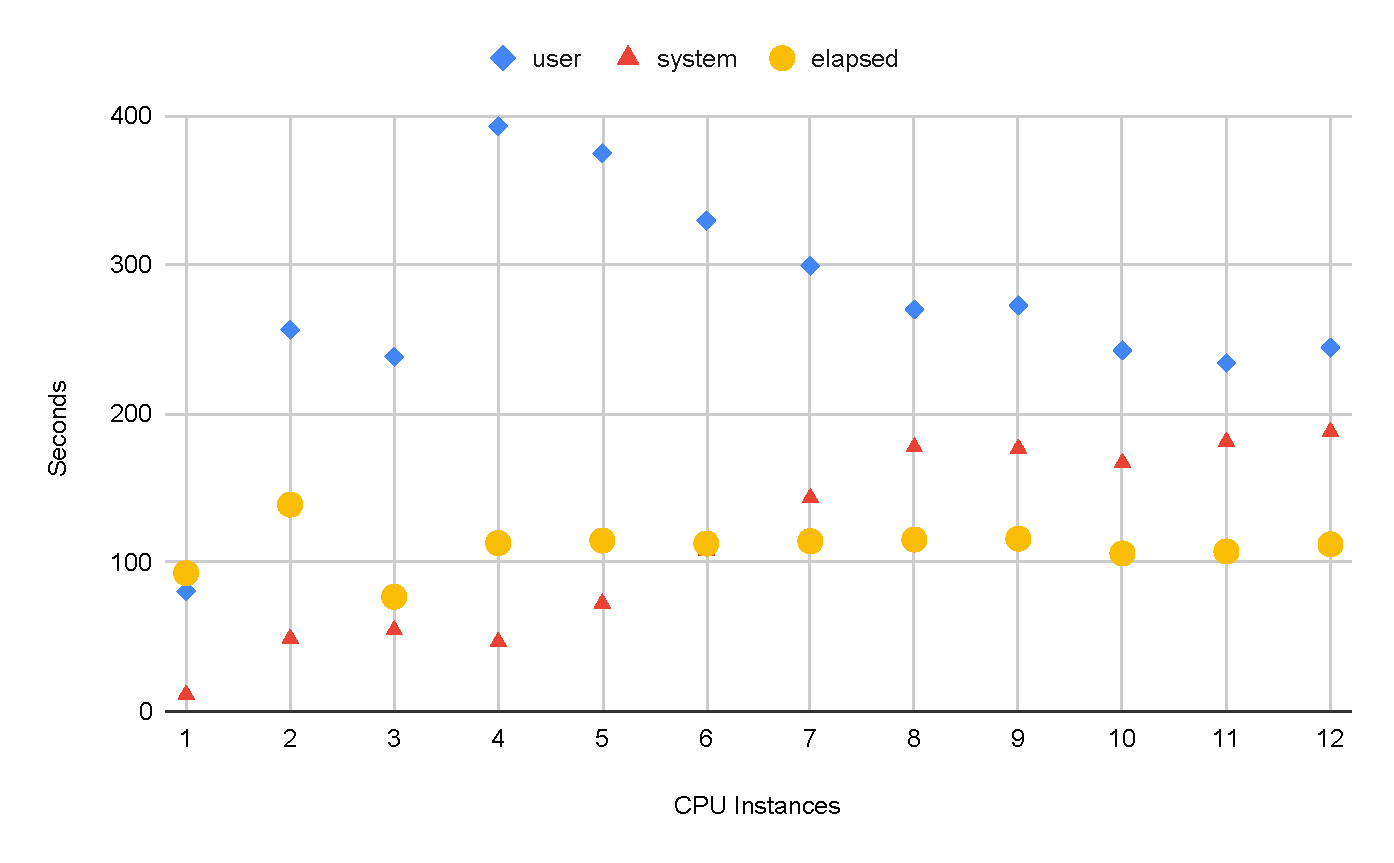
\includegraphics[width=1\linewidth,page=1]{experiments/speedup-clean.pdf}
    \caption{Métricas de tempo para execuções do \mfog com variação no número de processadores.}
    \label{fig:speedup}
  \end{minipage}
  \hfill
  \begin{minipage}{0.49\textwidth}
    \centering
    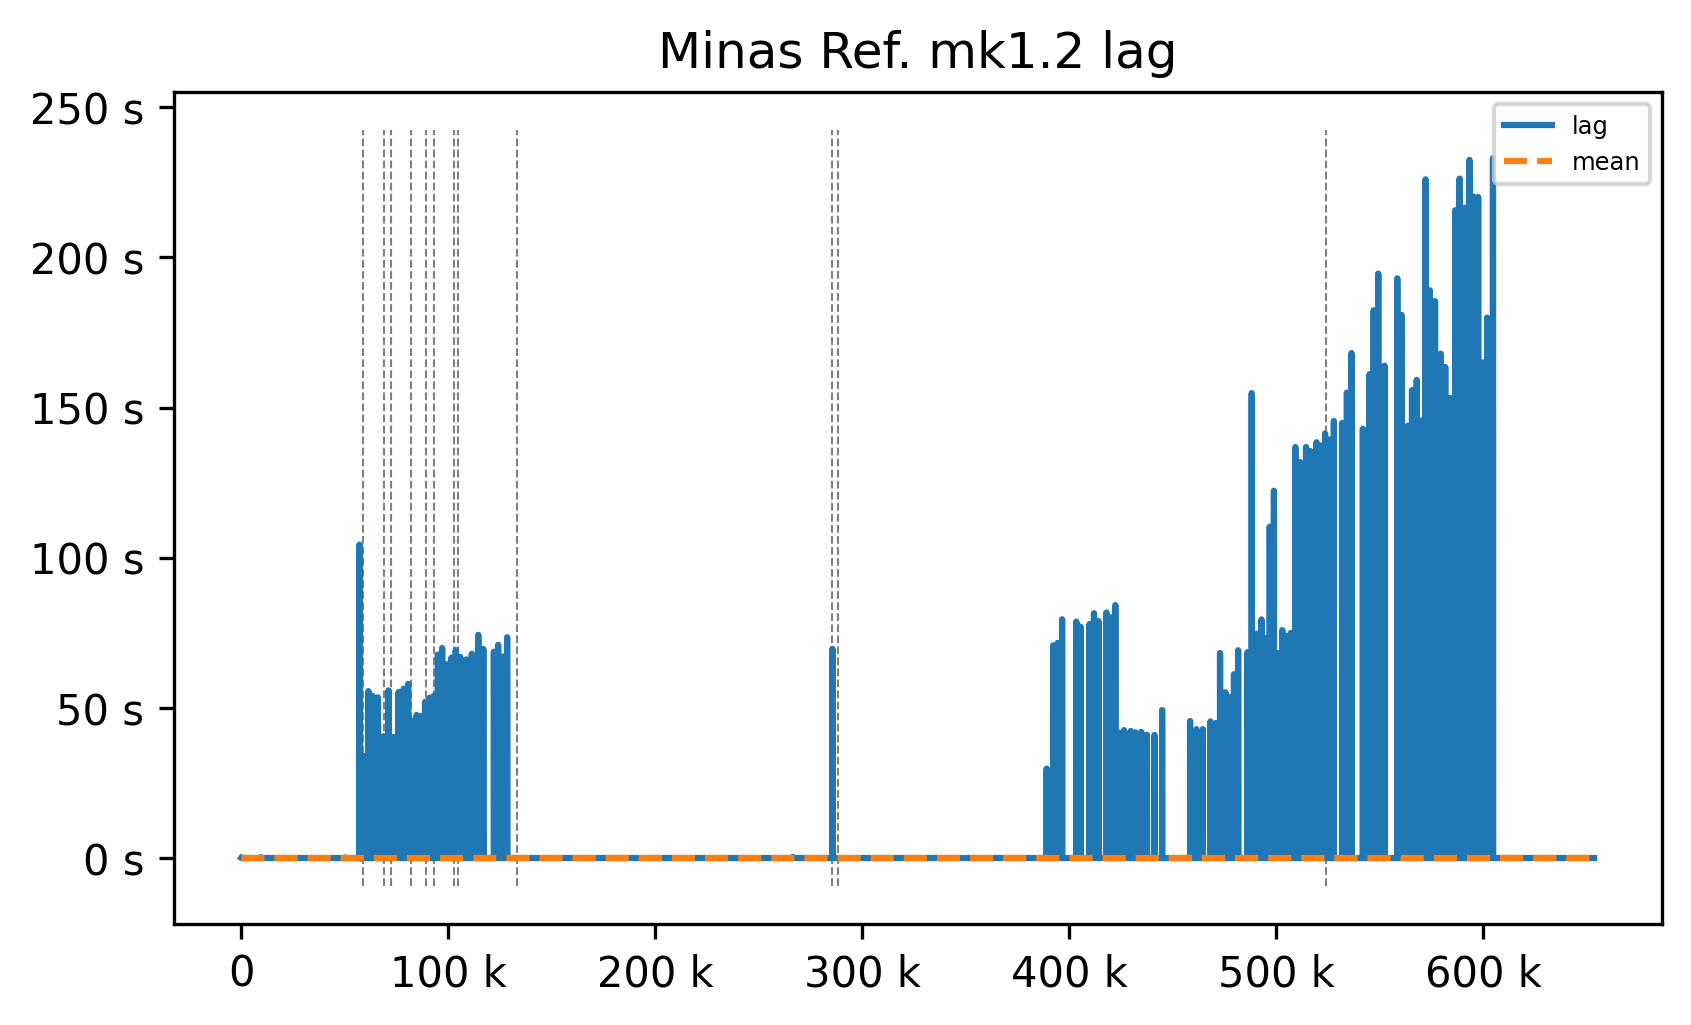
\includegraphics[width=1\linewidth]{experiments/lag-java.png}
    \caption{Visualização de Latência, Implementação de referência do algoritmo \minas.}
    \label{fig:lag-java}
  \end{minipage}
  % \hfill
  \vspace{5mm}
  \begin{minipage}{0.49\textwidth}
    \centering
    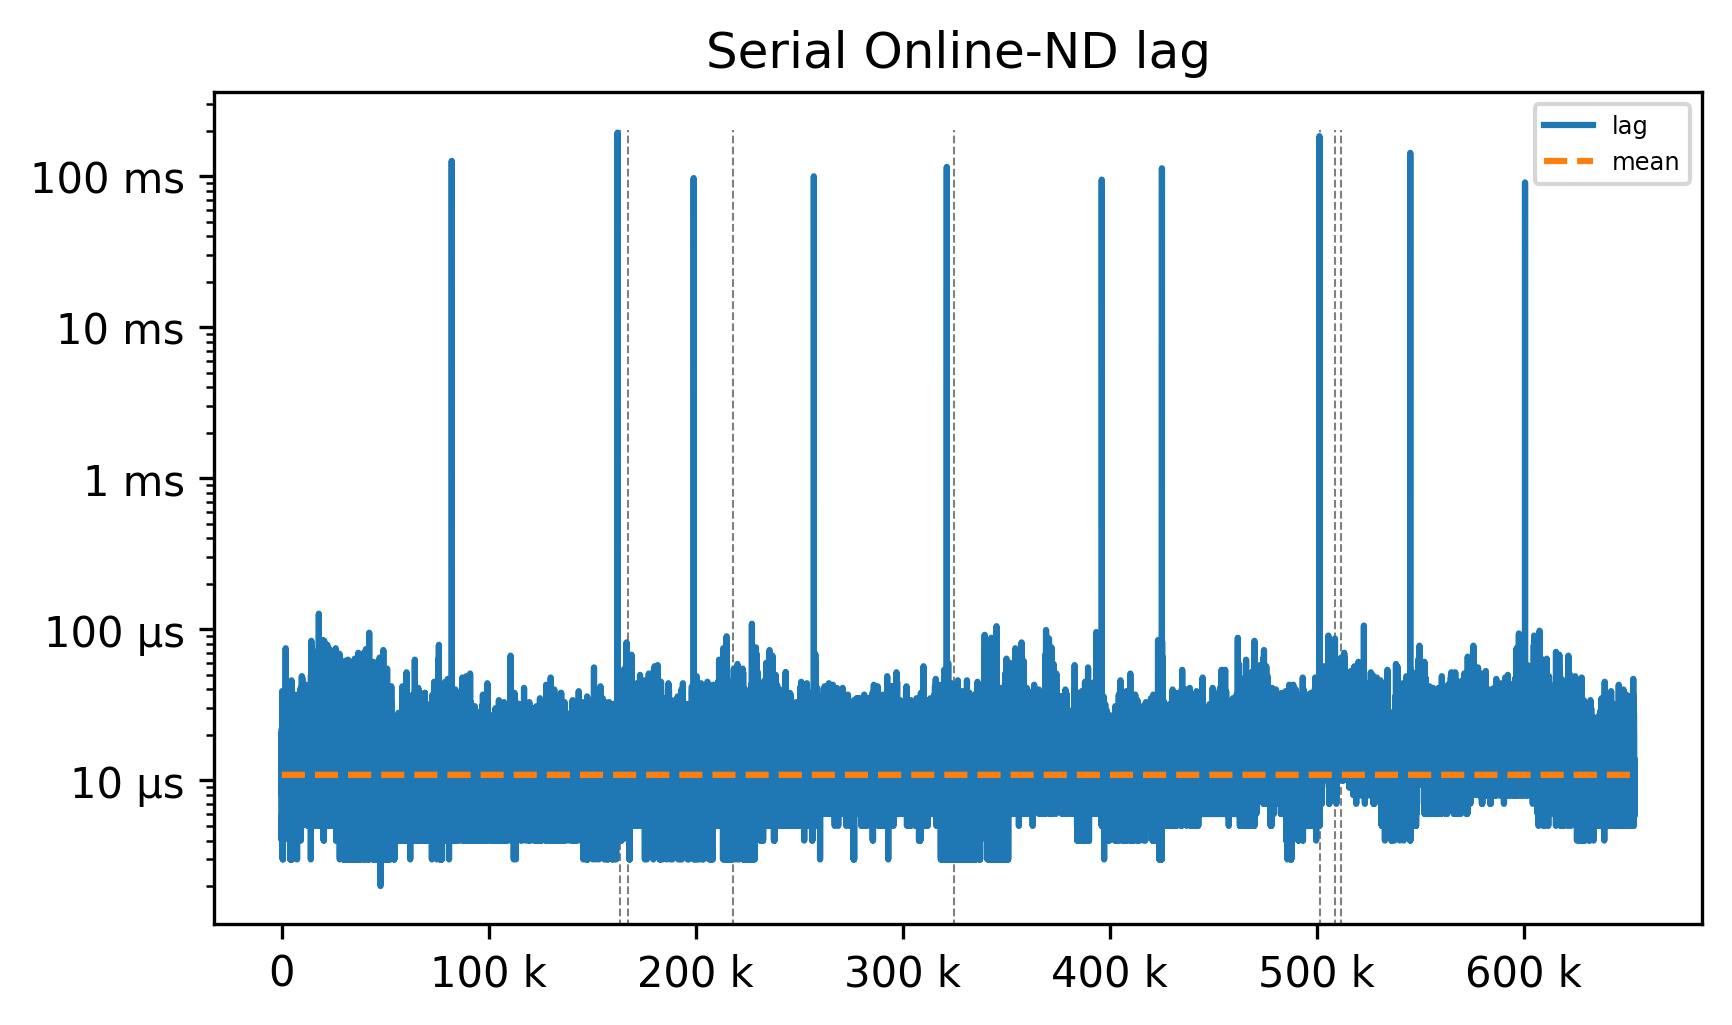
\includegraphics[width=1\linewidth]{experiments/lag-serial.png}
    \caption{Visualização de Latência na Implementação \emph{Serial} do algoritmo \minas usando funções do \mfog.}
    \label{fig:lag-serial}
  \end{minipage}
  % \vspace{5mm}
  \hfill
  \begin{minipage}{0.49\textwidth}
    \centering
    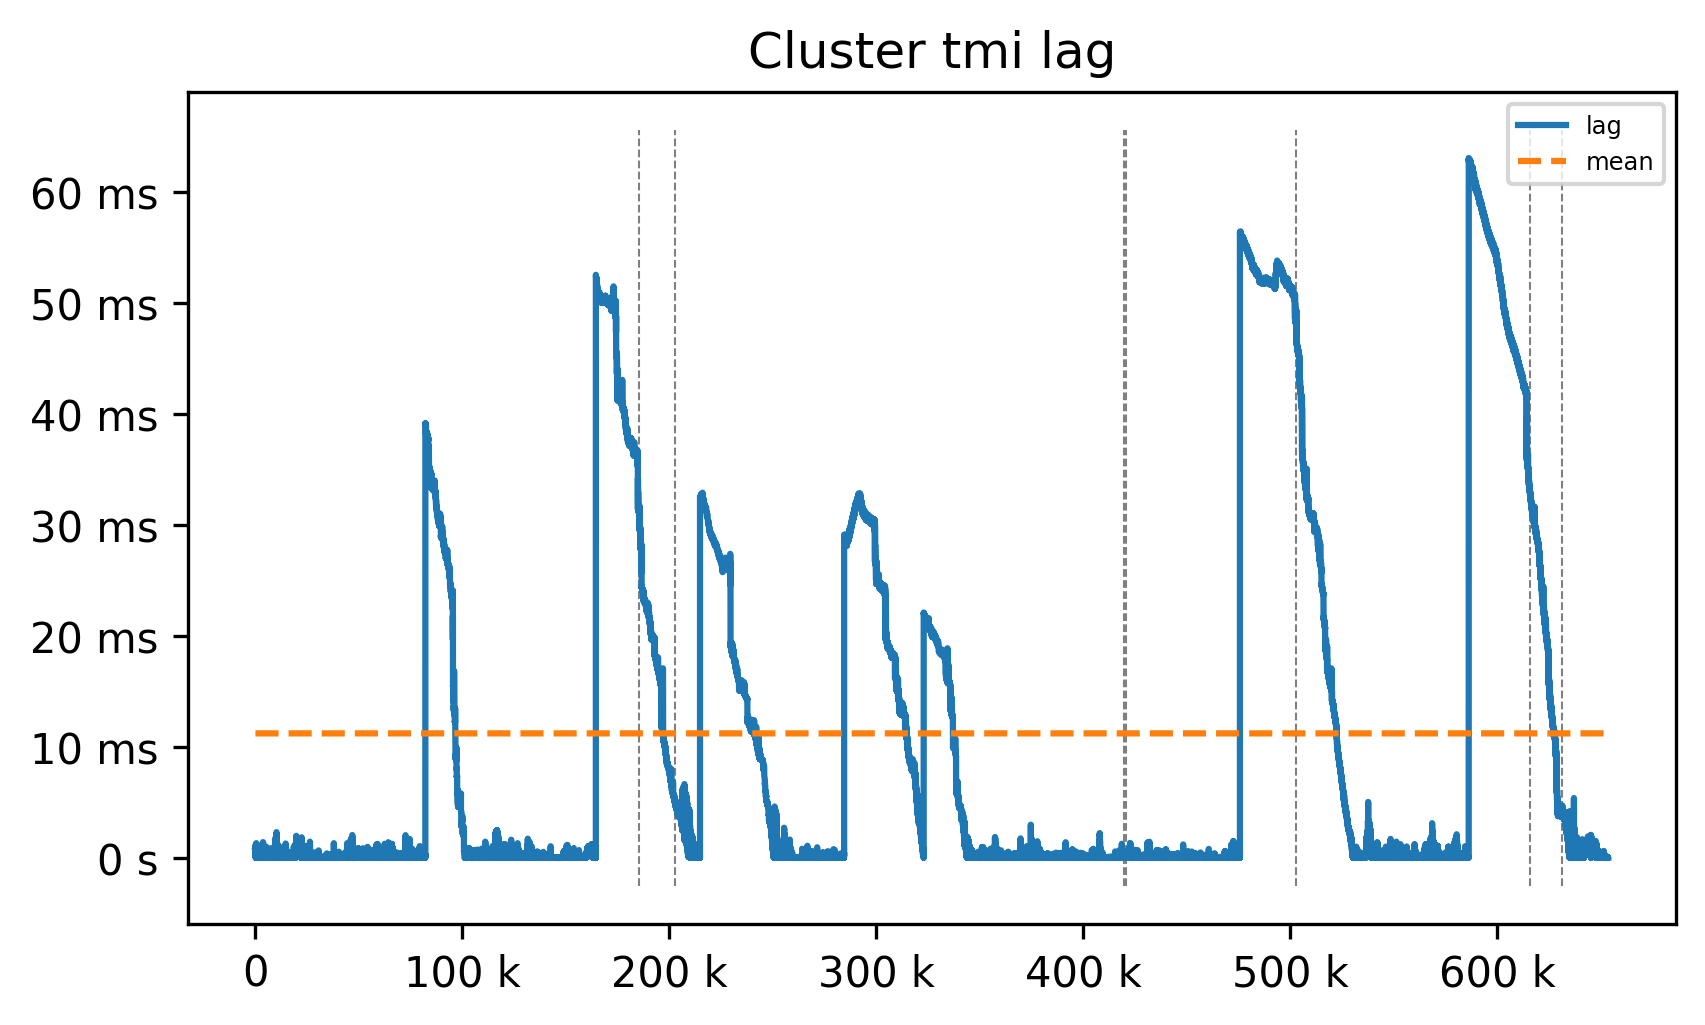
\includegraphics[width=1\linewidth]{experiments/lag-mfog.png}
    \caption{Visualização de Latência no \mfog.}
    \label{fig:lag-mfog}
  \end{minipage}
  % \caption{Experimentos adicionais \dataset \emph{Kyoto} Dez. 2015. Experimento fora do ambiente de \fog.}
  % \label{fig:lag}
\end{figure}

\FloatBarrier
\section{Conclusão}
\label{sec:exp-conclusao}

Os experimentos executados e os resultados obtidos demonstram que a
\acf{ND-DS} executada de maneira distribuída em ambiente de névoa (\fog) é
viável como parte de um \acf{NIDS} para redes \iot.


No entanto para aplicação em uma situação real, são necessárias otimizações
desde o \dataset de treinamento e avaliação, passando pelo algoritmo de detecção
de novidade, parâmetros do algoritmo e estratégias de paralelismo e
distribuição.
